\section{Test Reports}
\subsection{TR001: One Motor Test Rig}
\tr{T008}{AC008}{2}{BL012}{VPQ-21}
         {\shortstack[l]{GIVEN that we have a one motor test rig AND a microcontroller with a \\ working stabilizing code, WHEN we look at the test rig, THEN the motor \\ shall stay in the specified angle AND if we manually change angle;  the \\ motor shall adjust thrust accordingly.}}

\subsubsection*{\textsc{\medium Purpose}}
The purpose of TR001 is to gain information of how a single motor with a fixed pitch propeller can be stabilized in one axis. To conduct this test, and fulfil AC008, a motor mounted on an arm that can alter position in one axis. 

\subsubsection*{\textsc{\medium Test Setup}}
In Tab. \ref{tab:tab1} the equipment used conducting TR001 is displayed. 
\begin {table}[H]
    \begin{center}
    \caption {Test Equipment} 
    \label{tab:tab1} 
    \begin{tabular}{|l|l|l|}\hline 
        Brushless motor    & DJI E800   &\\ \hline
        ESC         & DJI E620S     &\\ \hline
        Power Supply & EA-PS 2342-06 B  & 20.1 V   \\ \hline
        Microcontoller & Arduino Nano ATmega328P \\ \hline
        IMU & MPU5060 \\ \hline
    \end{tabular}
    \end{center}
\end{table}

\noindent
In Fig. \ref{fig:onemotor} an illustration of the test setup for the One Motor Test Rig is displayed. The DJI E800 motor is mounted on an arm that can variate position in one axis. 

\begin{figure}[H]
    \centering
    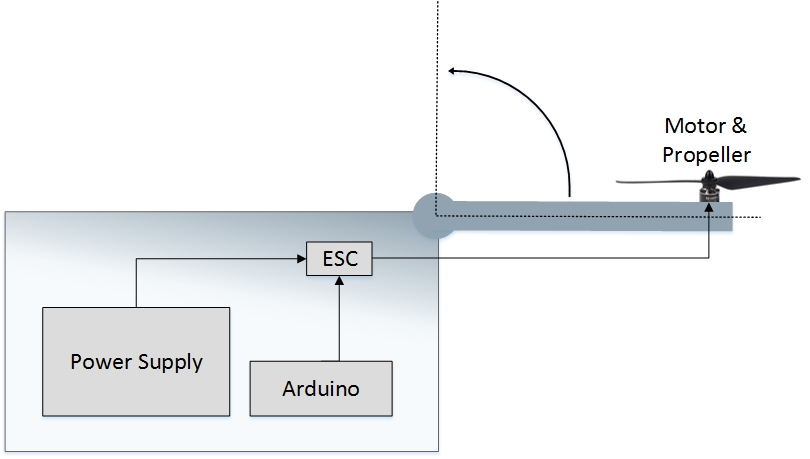
\includegraphics[width = 0.8\textwidth]{VAPIQ-PICTURES/TestSetup1}
    \caption{One Motor Test Rig Setup}
    \label{fig:onemotor}
\end{figure}

\noindent On the arm the MPU5060 is mounted, and this sensor transmits position data to the Arduino Nano. The Arduino Nano will then transmit a PWM signal to the ESC that equals desired thrust to the motor based on the measured sensor value. The amount of thrust is determined by the current position relative to desired position. 
\\\\
In Appendix A1 the code used for the One Motor Test Rig is displayed. For this test we used the $PID\_v1.h$ library to control and stabilize the arm. Before conducting this test we determined the most appropriate PID parameters by trial and error. These parameters are displayed in Tab. \ref{tab:tab2}.
\begin {table}[H]
    \begin{center}
    \caption {PID Parameters} 
    \label{tab:tab2} 
    \begin{tabular}{|l|l|}\hline 
        Kp         & 5  \\ \hline
        Ki         & 2   \\ \hline
        Kd         & 1  \\ \hline
    \end{tabular}
    \end{center}
\end{table}

\subsubsection*{\textsc{\medium Test Summary}}
\noindent
In code the desired angle (Setpoint = desired angle;) was set before transferring code to the microcontroller. When a desired angle was implemented and the code was compiled and transferred; the motor provided the appropriate thrust and the the motor arm moved to the wanted position. 
\\\\
When the arm was manually moved in a positive or negative direction relative to the desired angle the motor produced less or more thrust as intended.

\subsubsection*{\textsc{\medium Test Assessment}}
% [Enter a comprehensive assessment of your interpretation of how adequate the test was in light of how thorough the test plan said it should be? What wasn't tested well enough?]
%[Describe any variances between the testing that was planned and the testing that actually occurred.  Also, provide an assessment of the manner in which the test environment may be different from the operational environment and the effect of this difference on the test results
%[Provide a brief description of the unexpected results, problems, or defects that occurred during the testing.]
When using using libraries it is difficult to have an overview of how the code functions, unless the libraries are self composed. This may be a source of error.
\\\\
In this test, there were some measurement inaccuracy concerning the actual angle of the test arm and the angle input. This is due to the fact that we did not have a measuring device of actual arm angle. Also sensor instability was a reoccurring problem during the tests. Calibration and filtering of noise had to be done in order to achieve more stable results, and it still have potential for improvements.
\\\\
FIFO buffer overflow

\subsubsection*{\textsc{\medium Test Results}}
In this test the arm stayed in approximately the desired angle. In Tab. \ref{tab:tab3} the results of the One Motor Test Rig is displayed. 
\begin {table}[H]
    \begin{center}
    \caption {Test Results} 
    \label{tab:tab3} 
    \begin{tabular}{|l|l|l|}\hline 
        Test No.:  & Desired Angle:   & Comment:\\ \hline
        1         & 45    &  Arm stabilizes desired angle  \\ \hline
        2         & 30    &  Arm stabilizes desired angle   \\ \hline
        3         & 10    &  Arm stabilizes desired angle   \\ \hline
    \end{tabular}
    \end{center}
\end{table}
\newpage

%%%%%%%%%%%%%%%%%%%%%%%%%%%%%%%%%%%%%%

\subsection{TR002: Arduino Nano Computation Time}
\tr{T010}{AC013}{3}{BL033}{VPQ-106 VPQ-107}
         {\shortstack[l]{GIVEN that we have an Arduino Nano, WHEN we run a script, \\
                         THEN the microcontroller shall complete all computation within 20 ms}}
                         
\subsubsection*{\textsc{\medium Purpose}}
The purpose of TR002 is to determine if we can use an Arduino Nano as an on-board chip for our quadcopter. We will measure the time it takes for the control loops to compute. It is expected that the computation time is between 1 ms to 5 ms. 

\subsubsection*{\textsc{\medium Test Setup}}
In Tab. \ref{tab:tab4} the equipment used conducting TR002 is displayed. 
\begin {table}[H]
    \begin{center}
    \caption {Test Equipment} 
    \label{tab:tab4} 
    \begin{tabular}{|l|l|}\hline 
        Power Supply & EA-PS 2342-06 B     \\ \hline
        Microcontoller & Arduino Nano ATmega328P \\ \hline
        IMU & MPU5060 \\ \hline
        LED & \\ \hline
        Oscilloscope & \\ \hline
        \end{tabular}
    \end{center}
\end{table}

Quadcopters normally have two loops, one for the attitude control and one for the rate control.  Both these loops need to be completed within 20ms. This updating frequency is required to keep the quadcopter stable. Having a slow on-board chip can put serious restrictions on the project. The test consists of running a code which at the beginning of the loop lights a LED and at the end turns off the same LED. To measure the computational time, an oscilloscope was used to measure the time of one loop cycle.

\subsubsection*{\textsc{\medium Test Summary}}


\subsubsection*{\textsc{\medium Test Assessment}}
%[Enter a comprehensive assessment of your interpretation of how adequate the test was in light of how thorough the test plan said it should be? What wasn't tested well enough?]
%[Describe any variances between the testing that was planned and the testing that actually occurred.  Also, provide an assessment of the manner in which the test environment may be different from the operational environment and the effect of this difference on the test results
%[Provide a brief description of the unexpected results, problems, or defects that occurred during the testing.]


\subsubsection*{\textsc{\medium Test Results}}
In Tab. \ref{tab:tab5} the time needed for the Arduino Nano carry out its computations.  
\begin {table}[H]
    \begin{center}
    \caption {Computation Time} 
    \label{tab:tab5} 
    \begin{tabular}{|c|c|}\hline 
        Test No.: &  Result [ms]\\ \hline
        1. & 1.66 \\ \hline
        2. & 1.81 \\ \hline
        3. & 1.79 \\ \hline
    \end{tabular}
    \end{center}
\end{table}
The result is around what we expected from our it to be. It might bring
some limits on the project, but it should be doable. The worst case execution time of 1.81ms is not ideal. It is on the edge of what we need.  The advantages by using the Arduino Nano should be carefully examined vs.  the disadvantage of potential sacrifices done to the flight controller.  We might consider changing
to a more powerful on-board chip, especially for the variable pitch quadcopter.
Which we expect to be more computational heavy.

\newpage

%%%%%%%%%%%%%%%%%%%%%%%%%%%%%%%%%%%%%%

\subsection{TR003: 1-Axis Stabilization FPQ}
\tr{T011}{AC014}{3, 4}{BL033, BL032}{VPQ-106, VPQ-107}
         {\shortstack[l]{GIVEN that we have a one axis test rig AND a microcontroller with a\\ working
                         stabilization code, WHEN we look at the test rig AND the code \\ is running,
                         THEN The one axis test rig shall stay in the specified angle\\ AND if the
                         angle is manually changed; the motors shall adjust thrust \\accordingly. }}
                         

\subsubsection*{\textsc{\medium Purpose}}
The purpose of TR003 is to gain information of how to obtain stability, tune the controller and calibrate sensors. To do this, two motors with fixed pitch propellers is tested in 1-axis. To conduct the test, and fulfil AC014, one motor is mounted on each side of the test rig which pivots around its center allowing movement in 1-axis. 

\subsubsection*{\textsc{\medium Test Setup}}
In Fig. \ref{fig:testsetup3} an illustration of the test setup for the 1-axis test rig is displayed. 
\begin{figure}[H]
    \centering
    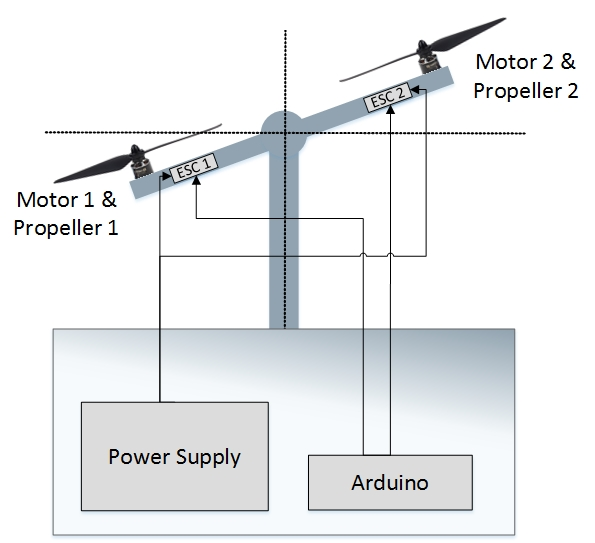
\includegraphics[width = 0.5\textwidth]{VAPIQ-PICTURES/TestSetup3}
    \caption{1-Axis Test Rig Setup}
    \label{fig:testsetup3}
\end{figure}

On the test rig a MPU9250 or 6050 is mounted, and the sensor transmits position data to the Arduino Nano. The Arduino Nano will then transmit a PWM signal to the ESC that equals desired thrust to the motors based on the measured sensor values. The amount of thrust is determined by the current position relative to desired position. To stabilize the test rig a self-developed P-control was implemented. 

In Appendix A2 the code for TR003 can be found. 

\subsubsection*{\textsc{\medium Test Summary}}
%[Include basic information about what was tested and what happened.]
All testing performed on the 1-axis test rig has been to understand and document how our stabilization algorithms and sensors are performing. The 1-axis rig has been used continuously for testing stability, sensors and code for fixed pitch. 

\subsubsection*{\textsc{\medium Test Assessment}}
% [Enter a comprehensive assessment of your interpretation of how adequate the test was in light of how thorough the test plan said it should be? What wasn't tested well enough?]
%[Describe any variances between the testing that was planned and the testing that actually occurred.  Also, provide an assessment of the manner in which the test environment may be different from the operational environment and the effect of this difference on the test results
%[Provide a brief description of the unexpected results, problems, or defects that occurred during the testing.]
During testing there has been problems with sensor stability when propellers have been mounted.

\subsubsection*{\textsc{\medium Test Results}}

The results obtained in this test rig has been valuable. It has helped to understand and fine tune code, stabilization algorithms and sensors continuously throughout the project.


\newpage
%%%%%%%%%%%%%%%%%%%%%%%%%%%%%%%%%%%%%%

\subsection{TR004: FPQ Hover Stabilization}
\tr{T012}{AC015}{4}{BL035 BL036}{VPQ-178 VPQ-184}
         {\shortstack[l]{GIVEN that we have assembled the FPQ, WHEN it is secured \\in testing rig AND we let the FPQ hover, THEN it shall stabilize itself.}}
\subsubsection*{\textsc{\medium Purpose}}
%hvorfor gjør vi dette?
The purpose of TR004 is to see how stable the quadcopter is in hover.

\subsubsection*{\textsc{\medium Test Setup}}
% hvordan gjør vi dette?
Fig. \ref{fig:ft1} and \ref{fig:ft2} shows the quadcopter secured on test table.

\begin{figure}[h]
        \centering
         \begin{minipage}[b]{0.495\textwidth}
            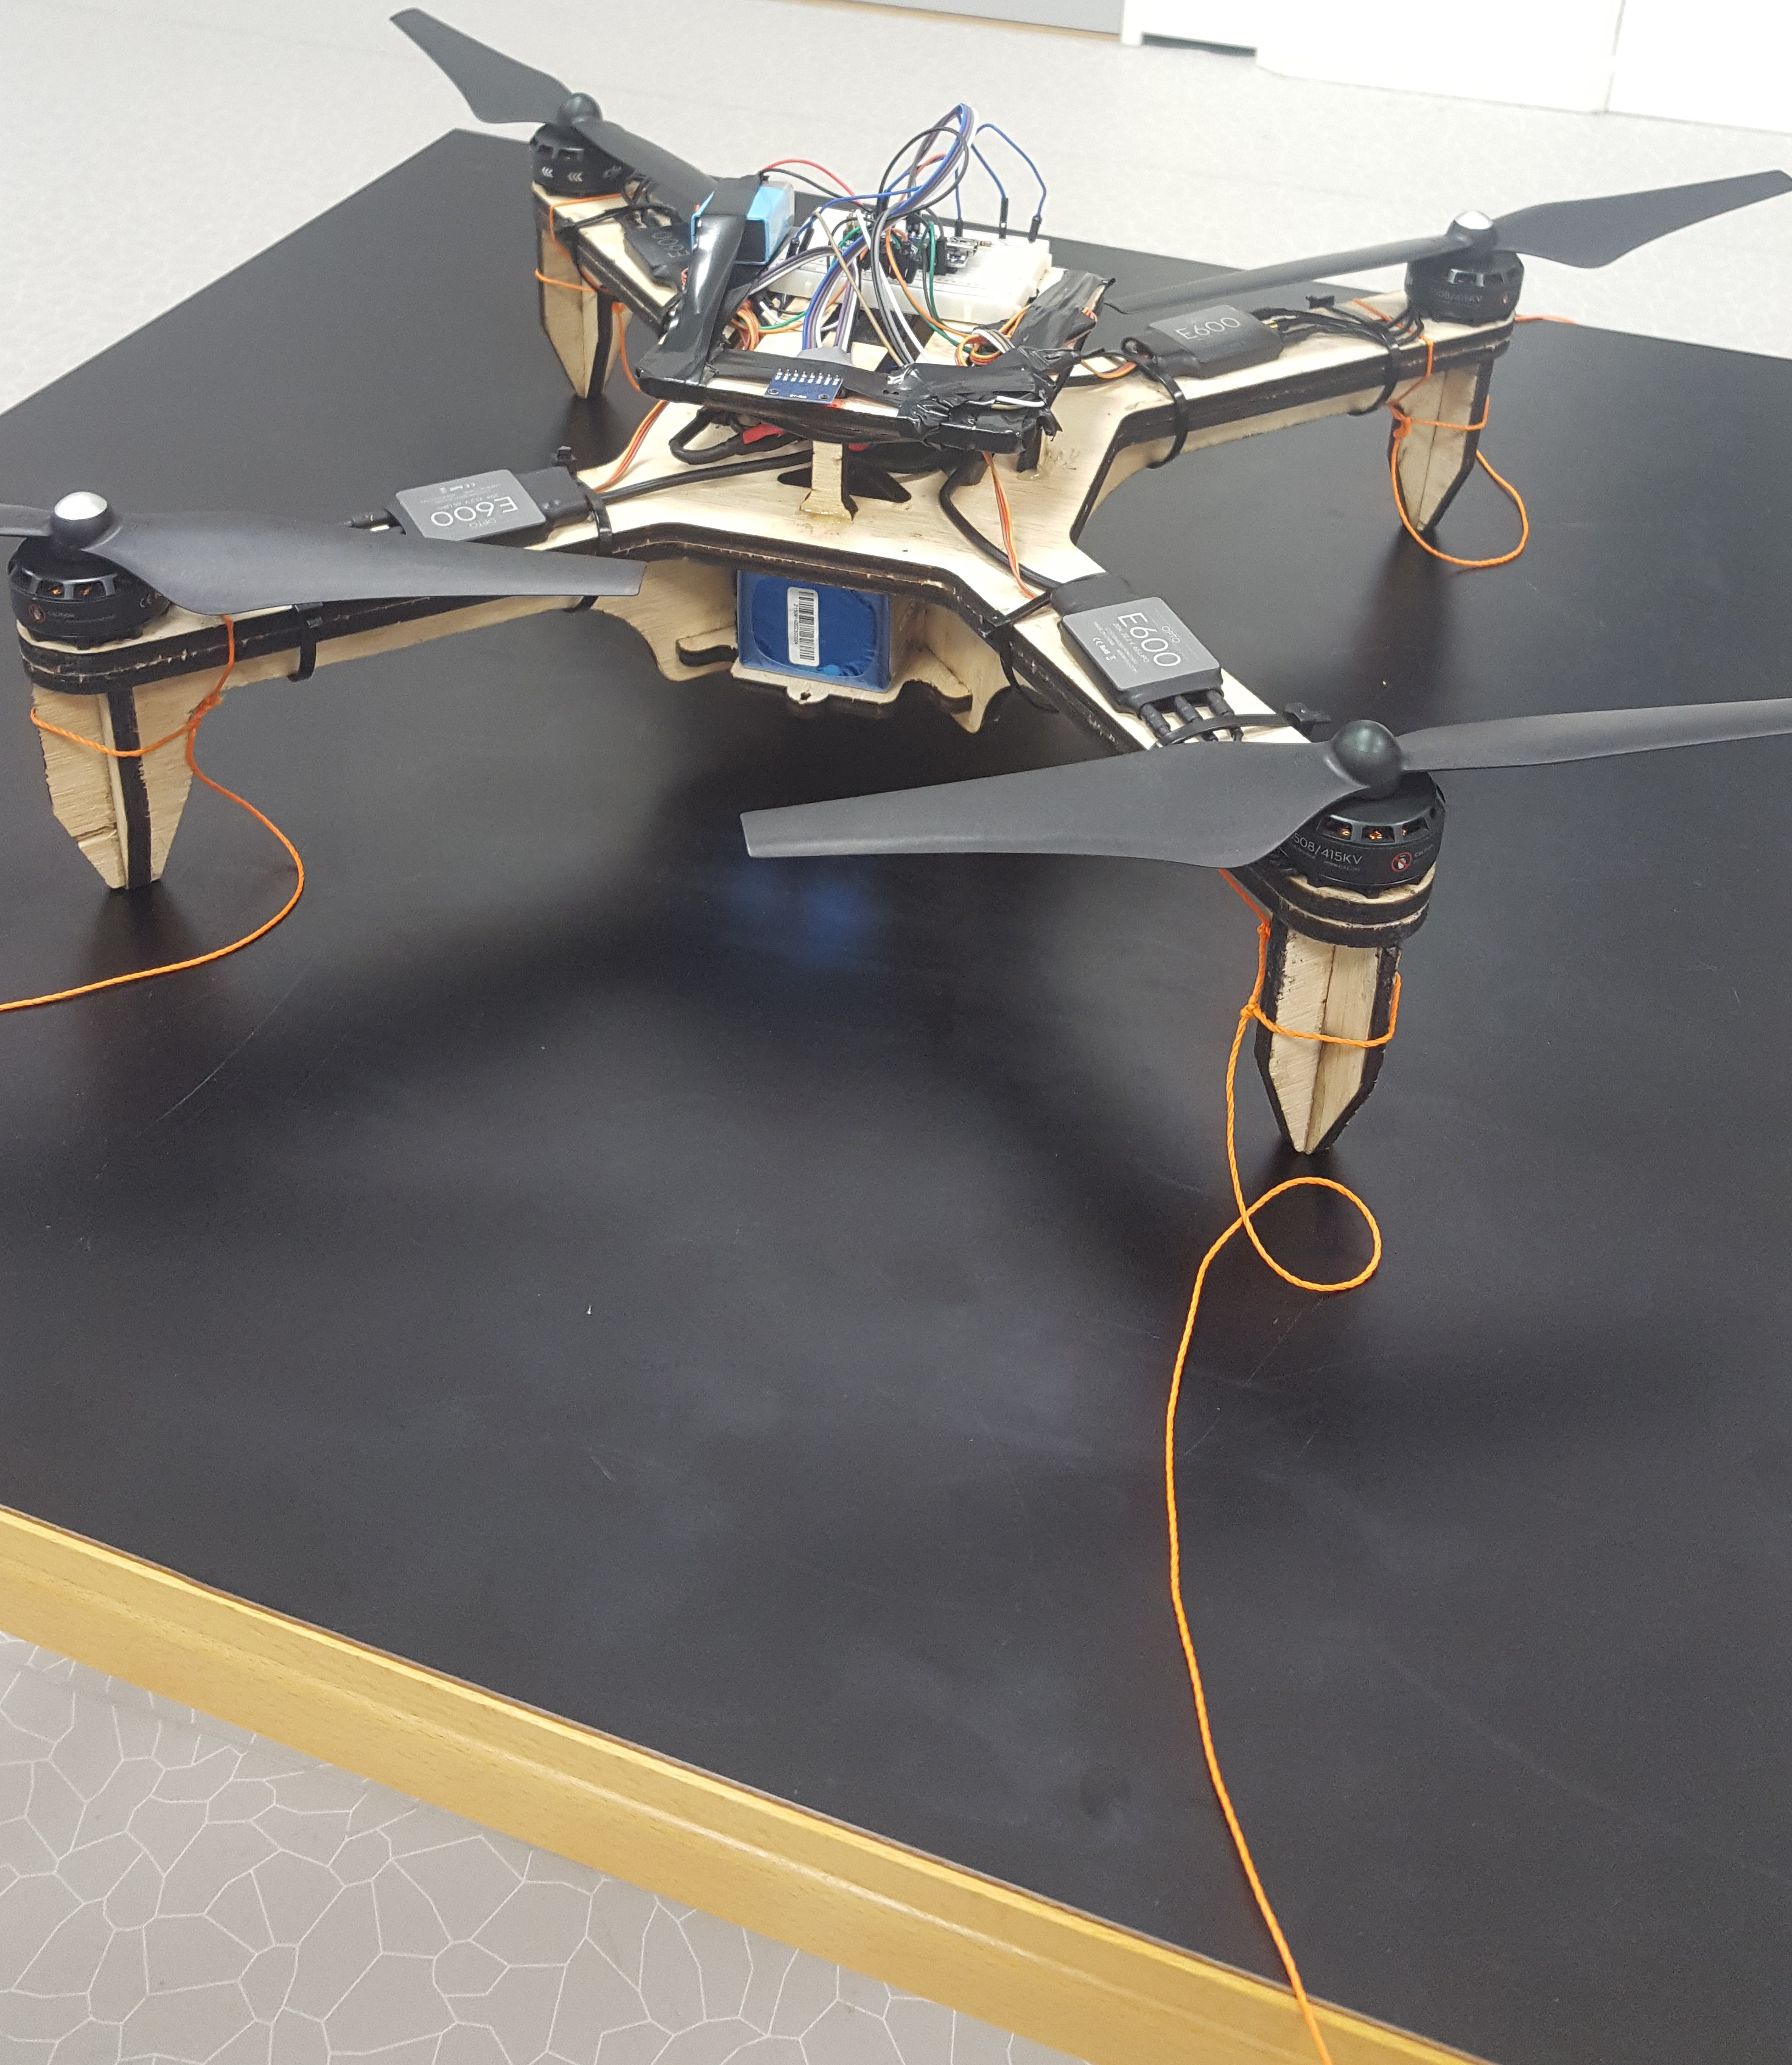
\includegraphics[width = 1\textwidth]{VAPIQ-PICTURES/flighttest2}
            \caption{Quadcopter tied to test table}
            \label{fig:ft1}
        \end{minipage}
        \hfill
        \begin{minipage}[b]{0.45\textwidth}
            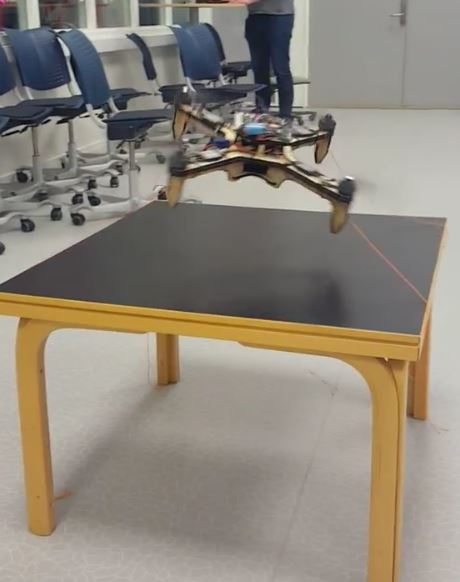
\includegraphics[width = 1\textwidth]{VAPIQ-PICTURES/flighttest}
            \caption{Quadcopter in flight}
            \label{fig:ft2}
        \end{minipage}
\end{figure}

\noindent In this test the stability of the quadcopter at hover is tested. The quadcopter was secured to a table by threads on each leg, ensuring that it could not uncontrollably fly away. In Appendix A4 the code used for TR004 can be found. 

\subsubsection*{\textsc{\medium Test Assessment}}
% egenvurdering av testen
% [Enter a comprehensive assessment of your interpretation of how adequate the test was in light of how thorough the test plan said it should be? What wasn't tested well enough?]

%[Describe any variances between the testing that was planned and the testing that actually occurred.  Also, provide an assessment of the manner in which the test environment may be different from the operational environment and the effect of this difference on the test results
%[Provide a brief description of the unexpected results, problems, or defects that occurred during the testing.]
The quadcopter was very unstable. The reason for this might be noise on sensor. Another factor may be when the quadcopter hits the end of the line a reaction force is experienced by the quadcopter, telling the sensors that a dramatic change in position has occurred, thus making the quadcopter overcompensate and react unstable. 
\\\\
At this point it can be concluded that a combination of these factors are the reason for unstable flight.

\subsubsection*{\textsc{\medium Test Results}}
%hva fikk vi ut av dette
The quadcopter was set to hover and did not stabilize.

\newpage
%%%%%%%%%%%%%%%%%%%%%%%%%%%%%%%%%%%%%%

\subsection{TR005: Motor Propeller Thrust Test Rig}
\tr{T013}{AC016}{4}{BL037}{VPQ-184}
         {\shortstack[l]{GIVEN that we have a test rig for motor and propeller combinations\\ AND a code where we can manually alter thrust, WHEN we look at test \\rig, THEN thrust in grams shall be displayed on weight.}}

\subsubsection*{\textsc{\medium Purpose}}
The purpose of TR005 is to evaluate the performance of the different motor and propeller combinations for fixed pitch. 

\subsubsection*{\textsc{\medium Test Setup}}
In Tab. \ref{tab:tab6} and \ref{tab:tab7} the equipment used conducting TR005.

\begin {table}[H]
    \begin{center}
    \caption {Test Equipment} 
    \label{tab:tab6} 
    \begin{tabular}{|c|}\hline 
        Power SupplyEA-PS 2342-06 B           \\ \hline
        Microcontoller Arduino Nano ATmega328P \\ \hline
        Motor \\ \hline
        ESC\\ \hline    
        \end{tabular}
    \end{center}
\end{table}

\begin {table}[H]
    \begin{center}
    \caption {Motor Propeller Combination} 
    \label{tab:tab7} 
    \begin{tabular}{|c|c|}\hline 
        Motor Test No. 1: & Motor Test No. 2:    \\ \hline
        DJI E600 & 3DR AC2836-358   \\ \hline
        12" propeller & 11" propeller \\ \hline
        ESC E620 & 3DR 20A-BEC\\ \hline
        415KV & 880KV\\ \hline
        \end{tabular}
    \end{center}
\end{table}
In Fig. \ref{fig:TestSetup5} an illustration of the test setup for the test rig is displayed.
\begin{figure}[H]
    \centering
    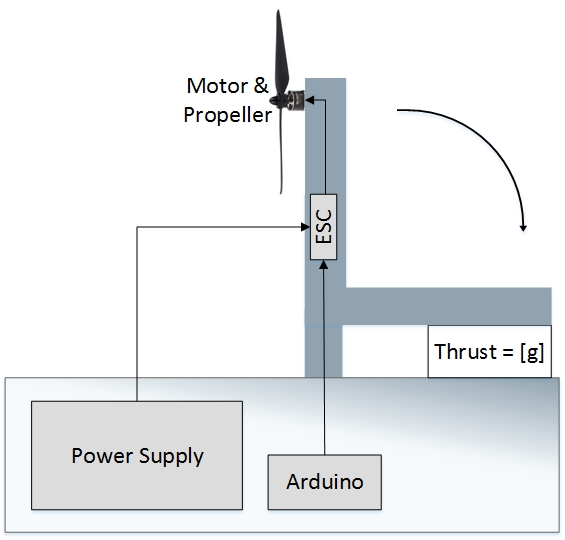
\includegraphics[width = 0.6\textwidth]{VAPIQ-PICTURES/TestSetup5}
    \caption{Thrust Test Rig Setup}
    \label{fig:onemotor}
\end{figure}

In this test we use a potentiometer to adjust the thrust. The potentiometer is mapped to have a value in microseconds between 1000 and 2000. Both motors were tested for several PWM values and the respective thrust values were noted.

In Appendix AX the code used for TR005 can be found. 

\subsubsection*{\textsc{\medium Test Assessment}}
% [Enter a comprehensive assessment of your interpretation of how adequate the test was in light of how thorough the test plan said it should be? What wasn't tested well enough?]
The testing rig gives a good indication of the actual thrust produced by the motor propeller combination. The rig may have some measuring inaccuracies due to the small variations in mechanical mounting, the difference in width of the mounting plate in comparison with the real quadcopter arm and the calibration of the weight.

\subsubsection*{\textsc{\medium Test Results}}
For our purposes, these tests have yielded the results needed in order to evaluate the performance of the motors and propellers.
                 
In Fig. \ref{fig:fpq3} and \ref{fig:fpq1} the result from this test is displayed. 

\begin{figure}[H]
    \centering
    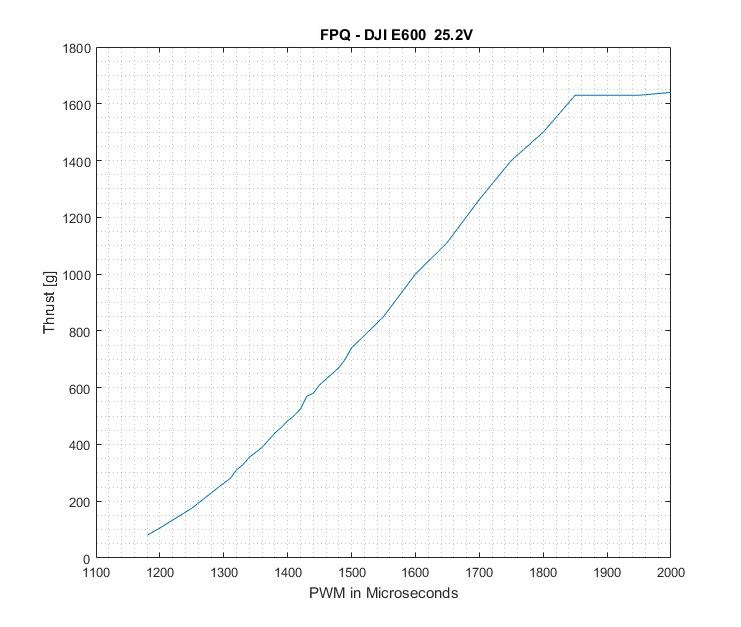
\includegraphics[width = 0.6\textwidth]{VAPIQ-PICTURES/FPQ3}
    \caption{DJI E600 with battery with PS25.2V}
    \label{fig:fpq3}
\end{figure}

\begin{figure}[H]
    \centering
    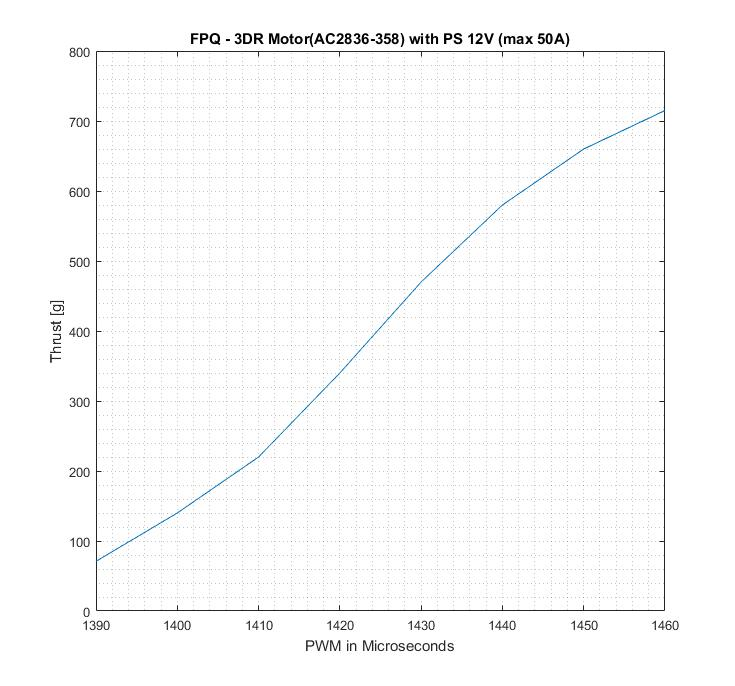
\includegraphics[width = 0.6\textwidth]{VAPIQ-PICTURES/FPQ1}
    \caption{3DR Motor(AC2836-358) with PS 12V}
    \label{fig:fpq1}
\end{figure}

Full test result table for TR005 can be found in Appendix B1.
 
 
\newpage       
%%%%%%%%%%%%%%%%%%%%%%%%%%%%%%%%%%%%%%
%%%%%%%%%%%%%%%%%%%%%%%%%%%%%%%%%%%%%%


\subsection{TR007: Variable Pitch Test - g/W and Servo Angle Input}
\tr{T015}{AC018}{5}{BL048}{VPQ-126}
         {\shortstack[l]{GIVEN that we have mounted a variable pitch mechanism to the thrust \\ test rig, WHEN we adjust the pitch and/or thrust, THEN the respective\\ thrust and current shall provide information about the efficiency of the \\ mechanism.}}


\subsubsection*{\textsc{\medium Purpose}}
The purpose of TR007 is to evaluate the efficiency of the variable pitch assembly as well as to provide information about the most efficient pitch angle. 

\subsubsection*{\textsc{\medium Test Setup}}
In Tab. \ref{tab:tab8} and \ref{tab:tab9} the equipment used conducting TR007 is displayed. 

\begin {table}[H]
    \begin{center}
    \caption {Test Equipment} 
    \label{tab:tab8} 
    \begin{tabular}{|c|}\hline 
        Power SupplyEA-PS 2342-06 B           \\ \hline
        Microcontoller Arduino Nano ATmega328P \\ \hline
        Motor \\ \hline
        ESC\\ \hline    
        \end{tabular}
    \end{center}
\end{table}

\begin {table}[H]
    \begin{center}
    \caption {Motor Propeller Combination} 
    \label{tab:tab9} 
    \begin{tabular}{|c|c|}\hline 
        Motor Test No. 1: & Motor Test No. 2:  \\ \hline
        3DR AC2836-358  & AXI 2208/26 \\ \hline
        9" propeller & 8" propeller \\ \hline
        3DR 20A-BEC & Multistar 12A - Turnigy \\ \hline
        880KV & 1420 \\ \hline
        \end{tabular}
    \end{center}
\end{table}


In ref{\ref{fig:VPM} 


\begin{figure}[H]
    \centering
    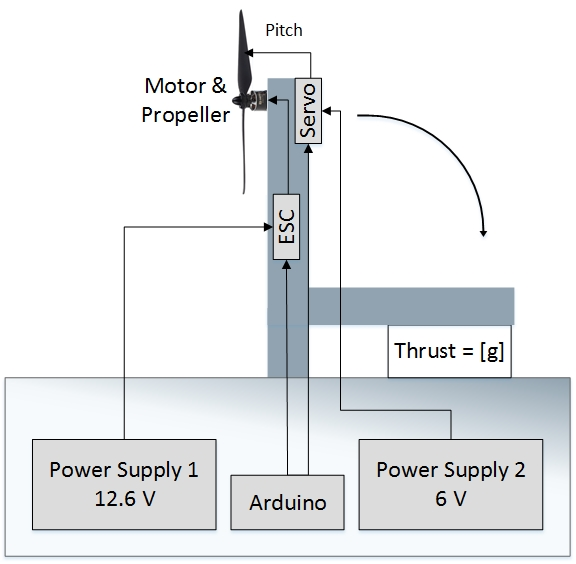
\includegraphics[width = 0.6\textwidth]{VAPIQ-PICTURES/TestSetup7}
    \caption{Thrust Test Rig Setup with VPM}
    \label{fig:VPM}
\end{figure}


\subsubsection*{\textsc{\medium Test Summary}}
%[Include basic information about what was tested and what happened.]
Also stress test on two servos

\subsubsection*{\textsc{\medium Test Assessment}}
% [Enter a comprehensive assessment of your interpretation of how adequate the test was in light of how thorough the test plan said it should be? What wasn't tested well enough?]
%[Describe any variances between the testing that was planned and the testing that actually occurred.  Also, provide an assessment of the manner in which the test environment may be different from the operational environment and the effect of this difference on the test results
%[Provide a brief description of the unexpected results, problems, or defects that occurred during the testing.]

\subsubsection*{\textsc{\medium Test Results}}
 For our purposes, these tests have yielded the results needed in order to evaluate the performance of the motors and propellers.
                 
In Fig. \ref{fig:vpm1} and \ref{fig:vpm2} the result from this test is displayed. 

\begin{figure}[H]
    \centering
    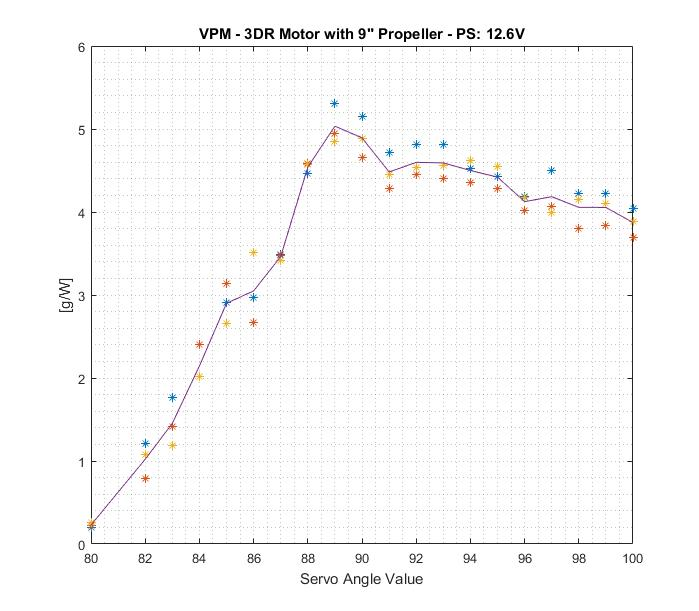
\includegraphics[width = 0.8\textwidth]{VAPIQ-PICTURES/VPM1}
    \caption{3DR Motor Efficiency}
    \label{fig:vpm1}
\end{figure}

\begin{figure}[H]
    \centering
    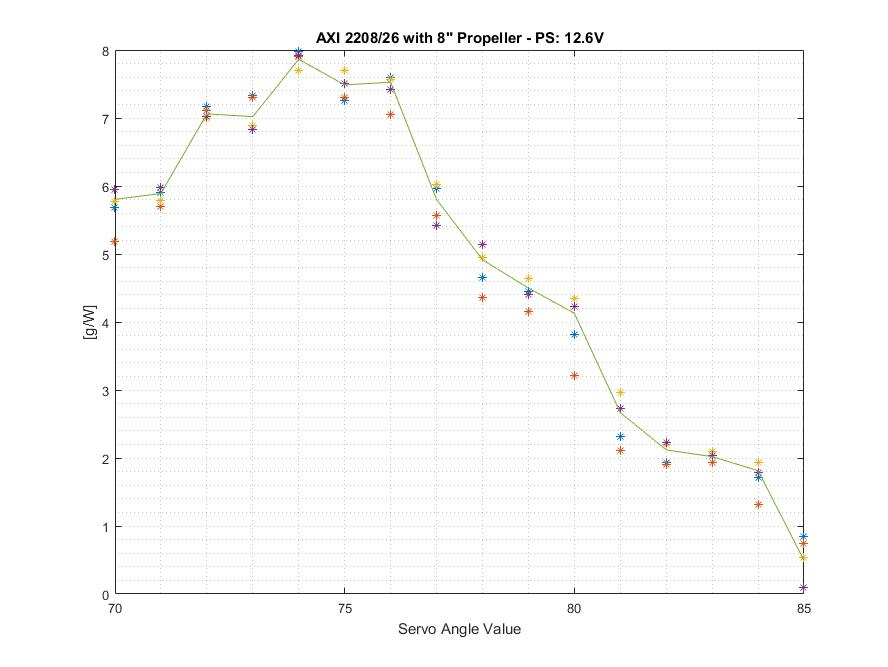
\includegraphics[width = 0.8\textwidth]{VAPIQ-PICTURES/VPM2}
    \caption{AXI Motor Efficiency}
    \label{fig:vpm2}
\end{figure}

Full test result table for TR005 can be found in Appendix B2.
         


         
